\chapter{Aineisto}%
\label{ch:aineisto}

Työn toteuttamiseen käytettiin cityscapes datasettiä \cite{Cordts2016Cityscapes}.


Datasetti pitää sisällään dispariteettidatan, sekä segmentaatiodatan.
Data on autosta stereokameralla kuvattua.
Malli on suunnattu automatisoituun liikenteeseen, ja siinä on paljon erilaisia kaupunkikuvia teiden varsilta.
Tämä tuottaa hankaluuksia lopputuloksen kanssa, sillä malli toimii reaalimaailmassa vain kaupunkikuvissa.
Kuitenkaan yleisempää disparteetti sekä segmentaatiomallia ei järkevästi löytynyt. 
Tämän ongelman olisi voinut kiertää käyttämällä erillisiä malleja segmentointiin sekä dispariteettiin. 
Kahden erialisen mallin yhdistäminen tuo kuitenkin enemmän riskejä.
Kahden mallin tapauksessa, jouduttaisiin joko luottamaan segmentaatiomalliin datan valmistelussa, 
tai kaikki data joduttaisiin käymään manuaalisesti läpi.

Data on kerätty erilaisista kaupunkiympäristöistä, ajoneuvon kyydistä kuvaten.
Tästä johtuen data on melko homogeenistä. Dataan on merkattu monia erilaisia segmentoituja kohteita, niinkuin ihmiisä polkupyöriä ja autoja. 
Tämän työn kannalta kuitenkin tärkeintä on, että kaikki liikkuvat kohteet on merkattu.
Kaikkia kuvia on tarjolla sekä vasemmasta että oikeasta kamerasta kuvattuna.
Data on tämän työn kannalta melko helposti työstettävää. Koska kaikki kuvat ovat ajoneuvosta otettuja, on kuvattava alue rajoittunut alueisiin joissa voi autolla ajaa.
Tämän kuitenkin tuottaa joitain rajoitteita datan käytössä, koska mallin käyttö tämän datasetin ulkopuolisen datan kanssa ei ole kovin helppoa ilman uudelleenkouluttamista.
Kaupungit joista data on kerätty on enimmäkseen sakalaisia kaupunkeja.
Ne ovat kuvatuilla alueilla usein hyvin tiheään rakennettuja. 
Tämä aiheuttaa, että suurella osalla syvyyskartoista on selkeät reunat.

Jotta datasta saataisiin kattavampaa, olisi hyvä keskittyä kuviin jotka on kuvattu muualta kuin kadulta.
Tämän avulla lopullista mallia voisi yleistää toimimaan myös muissa kuin autoteiden tunnistamisessa.
Toinen parantamiskohde dataan voisi olla kuvaaminen kaupunkien ulkopuolelta.
Tälläisiä kuvia ei tästä datasetistä löydy, koska sen pääkäyttökohde on segmentaatio datan käsittelyyn.

\begin{figure}[h]
\centering
\pdftooltip{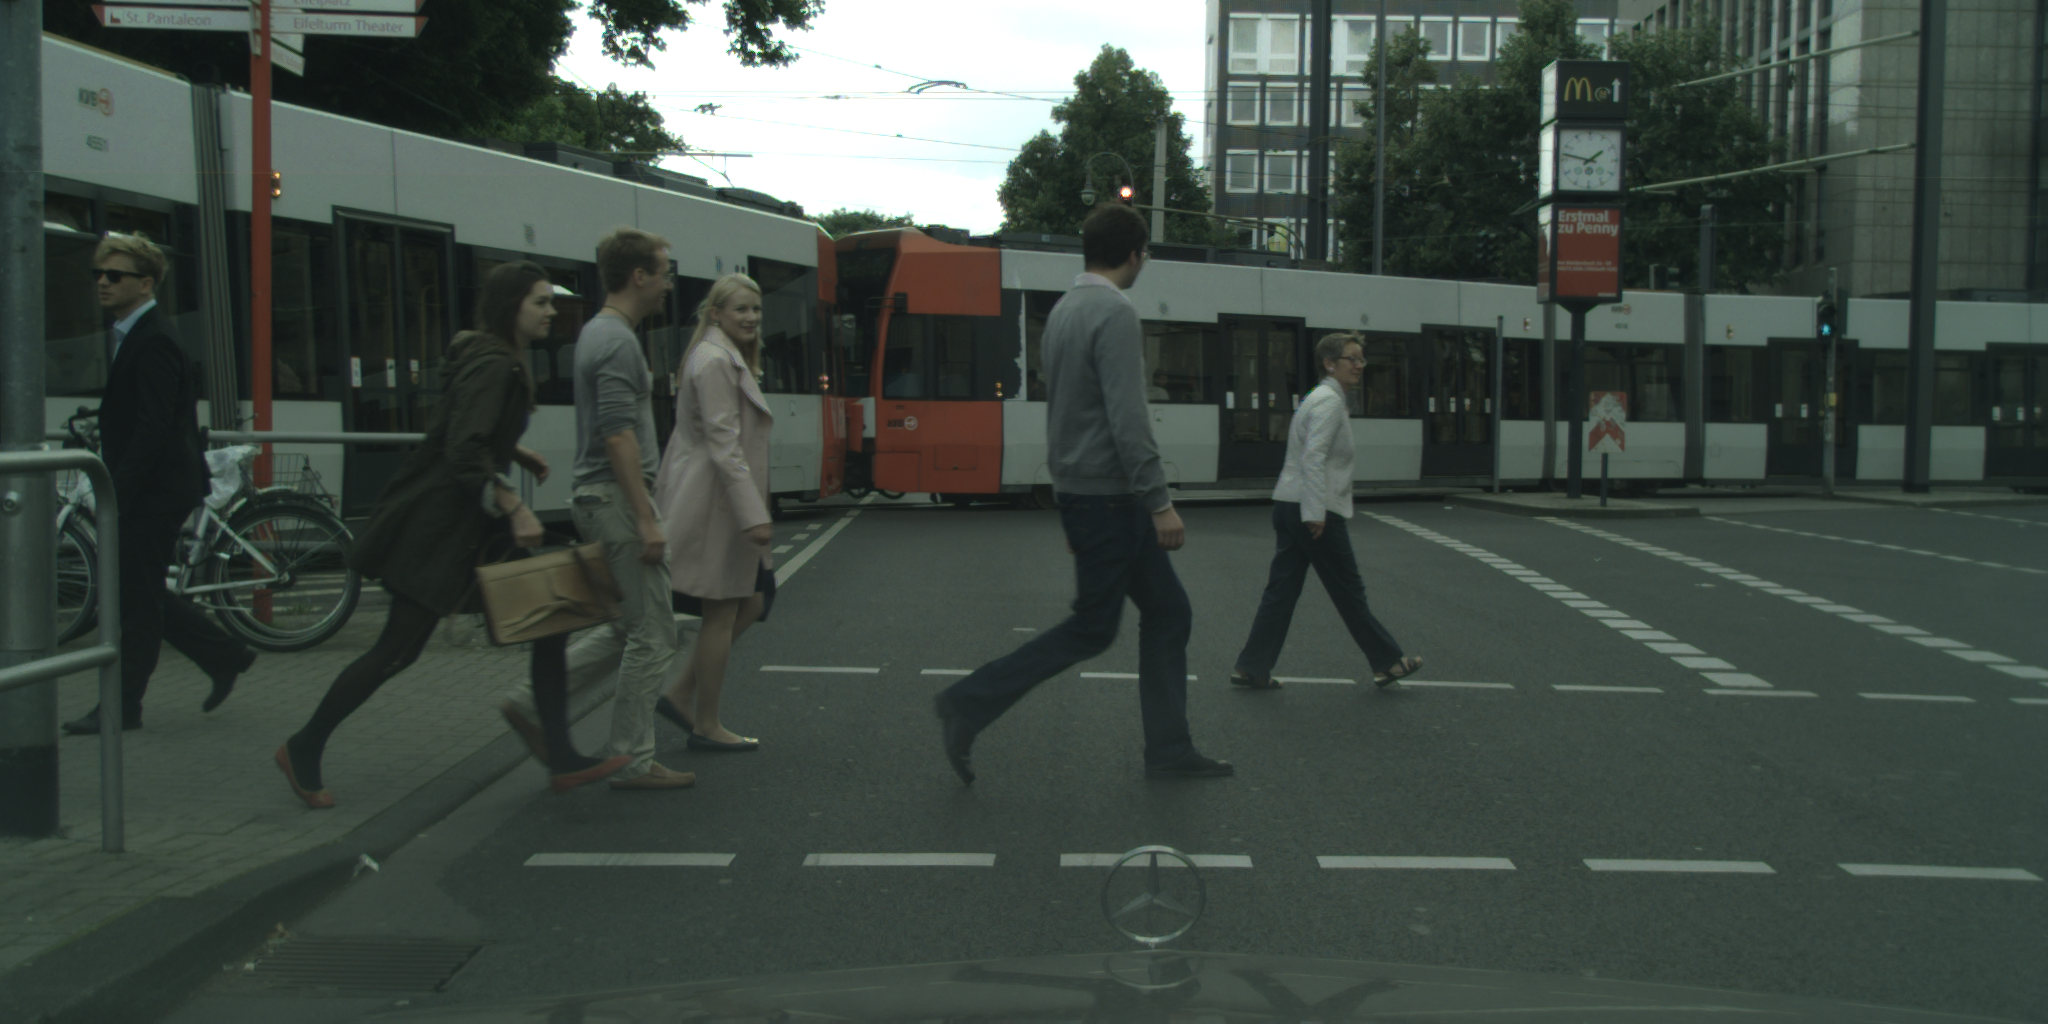
\includegraphics[width=\textwidth]{figures/extreme.png}}{extreme}
\caption{Esimerkki huonosta kuvasta}
\label{fig:extreme}
\end{figure}

    
Aineistossa on myös paljon kuvia jotka ovat "käyttökelvottomia" Kuva \ref{fig:extreme}.
Tämä kuva on hyvä esimerkki tilanteesta jossa edes ihminen ei pysty ilman laajaa taustatietoa arvelemaan mitä liikkuvien kohteiden takana olisi.
Ilman jonkinlaista ulkoista tietoa, tai datan generointia ei vain ole mahdollista tietää mikä haluttu totuus on.
Tämä tietysti on ongelma mitä tässä työssä halutaan ratkaista,
mutta lähtökohtaisesti paras lopputulos saadaan oikealla datalla.
Tälläinen datan generointi ja arvausten tekeminen toki onkin missä neuroverkot ovat omillaan.

